
This chapter will introduce Machine Learning (ML) concepts and techniques being explored in this work, namely the classification problem, neural networks and the Generative Adversarial Network architecture.

\section{Classification}

In Statistics and Machine Learning, a problem is defined as a classification problem when it consists in identifying which categories a population belongs to. An example might be identifying which race of domestic cat is shown in a picture containing a cat. An algorithm that implements classification is known as a classifier. The classifier works by analysing each observation into dependent variables and either mapping those to the categories or by comparing each observation to previous observations by means of a similarity function or loss function. 

Terminology between Statistics and Machine Learning tend to differ. In this work, we will be using the terminology found in Machine Learning, namely:

\begin{itemize}
	\item dependent variables are called features;
	\item categories are called classes;
\end{itemize}

In this work, we will not focus on a specific classification algorithm since ISA is not dependent on the algorithm used, only on the problem of classification.

\section{Neural networks}

% cito aqui ou não? perguntar
Neural networks, formally called \emph{artificial neural networks} (ANNs), are computational models inspired by networks of biological neurons \cite{Puri2016}. They are made up of multiple nodes called artificial neurons that map an input to an output based on mathematical operations. This model is used extensively in ML applications because of its perceived intelligent behaviour that come from the interactions between neurons.

\subsection{Artificial neuron}

The artificial neuron is the most basic block of an ANN. It maps inputs to an output in the given fashion:

\begin{equation} \label{eq:neuron_eq}
	y = f(\mathbf{w} \cdot \mathbf{x} + b),
\end{equation}

where the symbols are defined as:

\begin{equation} \label{eq:neuron_symbols}
	\begin{tabular}{ll}
		$\mathbf{x} = [x_1, x_2, \ldots, x_n]$ & Input vector;\\
		$\mathbf{w} = [w_1, w_2, \ldots, w_n]$ & Weights vector;\\
		$f$ & Activation function; \\
		$y$ & Neuron output.
	\end{tabular}
\end{equation}

The image \ref{fig:neuron} shows the artificial neuron model.

\begin{figure}[ht]
	\centering
	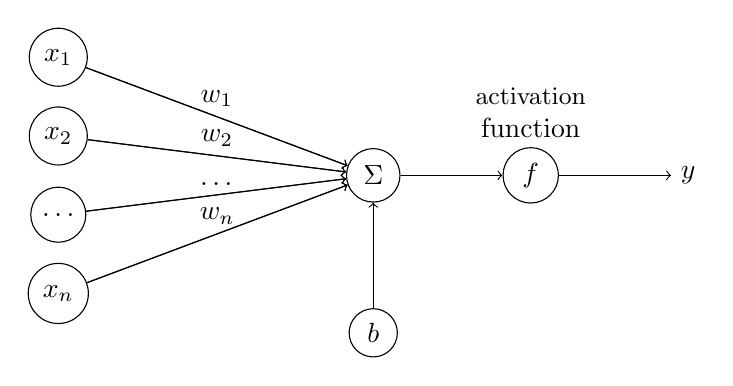
\begin{tikzpicture}
		% Neuron
		\node[circle, draw] (neuron) at (0, 0) {$\Sigma$};
		
		% Inputs
		\foreach \i/\name in {1/$x_1$, 3/$x_2$, 5/$\ldots$, 7/$x_n$} {
			\node[circle, draw] (input\i) at (-4, 4/2-\i/2) {\name};
			\draw[->] (input\i) -- (neuron);
		}
		
		% Weights (above)
		\foreach \i/\name in {1/$w_1$, 3/$w_2$, 5/$\ldots$, 7/$w_n$} {
			\draw[->] (input\i) -- (neuron) node[midway, above] {\name};
		}
		
		% Bias
		\node[circle, draw] (bias) at (0, -2) {$b$};
		\draw[->] (bias) -- (neuron);
		
		% activation function
		\node[circle, draw, label={[align=center]\small activation\\function}] (function) at (2, 0) {$f$};
		\draw[->] (neuron) -- (function);
		
		% Output
		\node (output) at (4, 0) {$y$};
		\draw[->] (function) -- (output);
	\end{tikzpicture}
	\caption{Model of a neuron.} \label{fig:neuron}
\end{figure}

This model of neuron is useful because it incorporates both the linear combination of input values and bias and the non-linearity of the activation function, which means it may function as a part of an universal function approximator \cite{HORNIK1989}.

\subsection{The network}

As said before, an ANN is a network of artificial neurons. Such network may be built by having the neurons configured in layers, having each neuron in a layer connected only to neurons in either preceding or following layers. Figure \ref{fig:fc_nn} shows a simple model of a fully-connected (a neuron in a layer connects to every neuron in the other layers) neural network, having 3 input nodes, 4 middle nodes (called a hidden layer) and 3 output nodes.

\begin{figure}[ht]
	\centering
		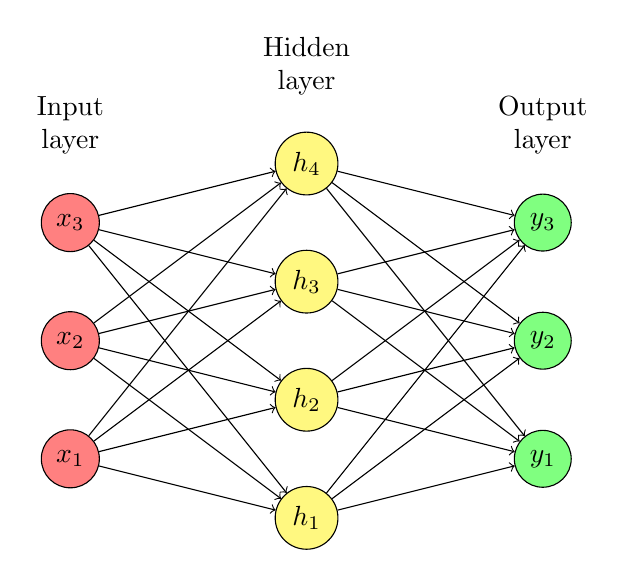
\begin{tikzpicture}[scale=1.5]
			% Input layer
			\foreach \i/\name in {1/$x_1$, 2/$x_2$, 3/$x_3$} {
				\node[circle, draw, fill=red!50] (input\i) at (0, \i) {\name};
			}
			\node[above, align=center] at (0, 3.5) {Input\\layer};
			
			% Hidden layer
			\foreach \i/\name in {1/$h_1$, 2/$h_2$, 3/$h_3$, 4/$h_4$} {
				\node[circle, draw, fill=yellow!50] (hidden\i) at (2, \i-1/2) {\name};
			}
			\node[above, align=center] at (2, 4) {Hidden\\layer};
			
			% Output layer
			\foreach \i/\name in {1/$y_1$, 2/$y_2$, 3/$y_3$} {
				\node[circle, draw, fill=green!50] (output\i) at (4, \i) {\name};
			}
			\node[above, align=center] at (4, 3.5) {Output\\layer};
			
			% Connections
			\foreach \source in {1, 2, 3} {
				\foreach \dest in {1, 2, 3, 4} {
					\draw[->] (input\source) -- (hidden\dest);
				}
			}
			
			\foreach \source in {1, 2, 3, 4} {
				\foreach \dest in {1, 2, 3} {
					\draw[->] (hidden\source) -- (output\dest);
				}
			}
		\end{tikzpicture}
		\caption{A model of a simple fully-connected neural network with 10 nodes.} \label{fig:fc_nn}
\end{figure}

\section{Generative Adversarial Networks}